\newpage
\section{Rep-Tiles Repeated}

\begin{teachingnote}
Materials:  Scissors and printed versions of the figures so that students can cut out already drawn ones.   
\end{teachingnote}

\begin{prob}
With a separate sheet of graph paper, draw and cut out the following polygons:
\[
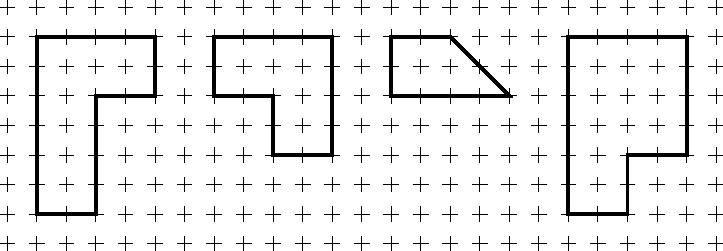
\includegraphics{../graphics/rep-4-tile1.pdf}
\]
Working with a partner, show that each of these polygons is a rep-4-tile.
\end{prob}

\begin{prob}
For each rep-tile above, compute the perimeter and area. In each case,
how does this relate to the perimeter and area of the larger polygon?
\end{prob}


\begin{prob}
With a separate sheet of paper, trace and cut out the following
polygons:
\[
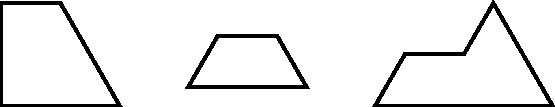
\includegraphics{../graphics/rep-4-tile2.pdf}
\]
Working with a partner, show that each of these polygons is a rep-4-tile.
\end{prob}


\begin{prob}
Explain why every rectangle whose sides have ratio $1:\sqrt{n}$ is a
rep-$n$-tile.
\end{prob}

\begin{prob}
Explain how you know that any polygonal rep-tile will tessellate the plane.
\end{prob}

\begin{prob}
Give an example of a polygon that tessellates the plane that is not a
rep-tile.
\end{prob}


\begin{prob}
Every tessellation made by rep-tiles will have \index{symmetry of
scale}\textbf{symmetry of scale}. What does it mean to have \textit{symmetry of scale}?
\end{prob}

\begin{prob}
Consider the tessellations made by rep-tiles you've seen so far. What
other symmetries do they have?
\end{prob}

\begin{prob}
Do you think you can have a tessellation that has symmetry of scale
but no other symmetries?
\end{prob}
